% Lo que debería contener este capítulo
% 
% Procesos de estampado
% Propiedades de materiales (Elasticidad / Plasticidad)
% Modelos constitutivos
% Método del elemento finito
% Teoría de contactos
% 
\chapter{Marco teórico}

\section{Procesos de formado}

El formado de metales incluye varios procesos de manufactura en los cuales se usa la deformación 
plástica para cambiar la forma de las piezas metálicas. La deformación es el resultado del uso de 
una herramienta que generalmente es un troquel para formar metales, mediante el cual se aplican 
esfuerzos que exceden la resistencia a la fluencia, induciendo una deformación plástica 
~\cite{groover2007}\\.

Normalmente, se aplica un esfuerzo de compresión para deformar plásticamente el metal, no obstante, 
algunos procesos de formado estiran, cortan o doblan el metal. Para que un metal sea adecuado 
como materia prima en un proceso de formado, este debe poseer ciertas propiedades mecánicas, 
tales como una baja resistencia a la fluencia y alta ductilidad, para facilitar la deformación 
plástica. Además, debe tenerse en cuenta el factor de la temperatura, mismo que determina 
la clasificación de trabajo en frío y caliente (referente a la temperatura de cristalización). 
También la velocidad de formación y el fenómeno de fricción entre la pieza metálica y el herramental 
son factores adicionales que afectan el desempeño del formado de metales.\\

\subsection{Tipos de formado}

Los procesos de formado se pueden clasificar en dos categoría generales, a saber: procesos de 
deformación volumétrica y procesos de trabajo de láminas metálicas.~\cite{groover2007}\\

Los \textbf{procesos de deformación volumétrica} se caracterizan por deformaciones significativas 
que derivan en grandes cambios de forma, y la relación entre el área superficial y el volumen 
de trabajo es relativamente pequeña. Algunos tipos de formado que entran dentro de esta 
clasificación son: rolado, forjado, extrusión y estirado.\\

Los \textbf{procesos de trabajo de láminas metálicas} son operaciones de formado o preformado 
de láminas, tiras y rollo de metal. La razón entre el área superficial y el volumen del material 
inicial es alta, por lo que esta relación es un medio útil para distinguir la deformación 
de los procesos descritos anteriormente. Estas operaciones se ejecutan siempre en frío y 
se utiliza un herramental compuesto en la mayoría de los casos de un conjunto de formadores, 
conocidos comúnmente como punzones y matrices en el ámbito industrial. Se pueden 
distinguir de manera general tres tipos de operaciones que entran en esta clasificación: 
doblado, estirado y corte.\\

En este caso centraremos el interés en esta última clasificación, puesto que el proceso 
de formado del tubo se realiza utilizando una combinación de corte-doblado.

\subsection{Herramentales (troqueles)}

Los herramentales utilizados en los procesos de formado (comúnmente llamados troqueles) son 
construidos teniendo en cuenta algunos aspectos elementales, a saber ~\cite{marin2009}:

\begin{enumerate}
\item Trabajo a realizar 
\item Características de la prensa
\item Material a troquelar
\item Número de piezas a producir
\end{enumerate}

\subsubsection{Tipos de troqueles}

A medida que aumentan los requerimientos del trabajo, la capacidad de las prensas, las exigencias 
de los materiales y la necesidad de producir más y mejor, también se conciben los diseños de 
troqueles con mayor complejidad y desarrollo. En ese sentido, los troqueles se pueden clasificar 
en simples, compuestos y progresivos.\\

\textbf{Simples}: estos troqueles permiten realizar solamente una operación por cada golpe o 
ciclo de la prensa, lo cual implica una bajo volumen de producción y productividad, y 
siendo normalmente necesario el uso de más de un herramental para terminar el producto.\\

\textbf{Compuestos}: permiten aprovechar la fuerza ejercida por la prensa realizando dos 
o más operaciones en cada golpe, agilizando el proceso y elevando en cierto punto 
la productividad.\\

\textbf{Progresivos}: son troqueles complejos y de gran desarrollo. Constan de una 
cantidad considerable de etapas, en cada uno de ellos se modifica la lámina con una secuencia 
establecida durante el diseño y acorde a los requerimientos del producto, de tal manera 
que al final se obtiene una o varias piezas terminadas. Naturalmente son altamente productivos, 
aunque su mantenimiento y operación es más compleja que en los casos anteriores.

\subsubsection{Componentes de un troquel}

Los componentes de un troquel varían dependiendo del tipo, pero típicamente hay elementos 
que se encuentran en casi todos los troqueles y que cumplen con funciones específicas 
en el proceso de formado.\\

\textbf{Base superior}. Contiene en su interior todas las placas y elementos que sostienen 
los punzones del troquel, está anclada a la prensa. Algunos elementos alojados en 
la parte superior son: placa porta-punzones, punzones, sufrideras, postes, pisadores, resortes, 
entre otros elementos adicionales.\\

\textbf{Base inferior}. Es el elemento sobre el cual van montados todos los componentes 
que hacen la parte de la matriz, y a su vez, está fuertemente sujeta en la bancada 
de la prensa durante la fase de trabajo. Algunos de los elementos contenidos en 
la base inferior son: placa  porta-matrices, guías, sufrideras, topes de avance, entre 
otros.\\

\textbf{Sufrideras}. La función básica de las placas superior e inferior de choque o sufrideras 
consiste en absorber sobre su superficie los sucesivos golpes de los elementos en el troquel. 
Estos impactos se producen cada vez que los punzones transforman la lámina con la matriz. Cuando 
el punzón impacta contra el material, la resistencia que opone este es transmitida a la 
superficie de las sufrideras sobre las que se apoyan las placas porta matriz y porta punzones. 
Estas placas están construidas en materiales ya templados y que conservan su tenacidad y cohesión, 
uno muy empleado es el acero SAE/AISI 1045.\\

\textbf{Porta punzones}. La finalidad de la placa porta punzones es la de alojar y fijar en 
su interior todos los punzones que lleve la matriz. Estos punzones pueden ser de cualquier 
tipo o tamaño pero han de tener una sola carcterística en común: deben estar firmemente 
sujetos y guiados en el interior de dicha placa impidiendo que puedan moverse o desprenderse.\\

\textbf{Porta matriz}. La placa porta matrices aloja y posiciona en su interior todos 
los elementos de pequeñas dimensiones que lleve la propia matriz, de esta manera dichos componentes 
quedarán ajustados en su interior.\\

\textbf{Placa pisadora}. Durante el movimiento descendente del troquel, la placa pisadora presiona 
la lámina dejándola inmovilizada antes de que los punzones lleguen a tocarla y mientras penetran 
el material y lo transforman. Una vez cortada la lámina, la función de la placa es mantener la 
pieza bien sujeta hasta que los punzones hayan salido de ella, de lo contrario, los punzones 
la arrastrarían hacia arriba sujeta a ellos, con el riesgo de fractura.\\

\textbf{Punzones}. Los punzones tienen por objeto realizar las máximas transformaciones en la lámina 
a fin de obtener piezas con una calidad acorde a las medidas requeridas, hay tanto tipos de estos 
como variantes del troquelado.\\

\textbf{Matrices}. Las matrices son los elementos complementarios a los punzones, tienen la forma 
negativa de estos.

\begin{center}
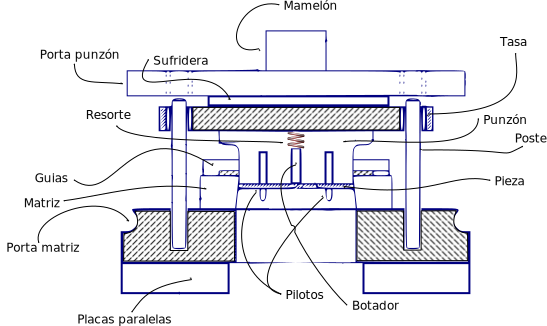
\includegraphics[scale=0.3]{src/ch2/componentes_troquel.png}
\captionof{figure}{Componentes de un troquel. \textit{Fuente:} ~\cite{wikiTroquel2008}}
\label{fig:componentes_troquel}
\end{center}



\section{Mecánica de sólidos}

\subsection{Relaciones constitutivas}

En el caso de un sólido tridimensional isotrópico la relación esfuerzo-deformación está dada por la Ley de Hooke, 
expresada en términos matemáticos como:

\begin{equation}\label{eq:ecdef}
\vec{\varepsilon} = 
\left\{\begin{matrix}
\varepsilon_{xx} \\ \varepsilon_{yy} \\ \varepsilon_{zz} \\ \varepsilon_{xy} \\ \varepsilon_{yz} \\ \varepsilon_{zx}
\end{matrix}\right\} = 
\left[ C \right] \vec{\sigma} + \vec{\varepsilon_0} = 
\left[ C \right]
\left\{\begin{matrix}
\sigma_{xx} \\ \sigma_{yy} \\ \sigma_{zz} \\ \sigma_{xy} \\ \sigma_{yz} \\ \sigma_{zx}
\end{matrix}\right\} + 
\left\{\begin{matrix}
\varepsilon_{xx}_0 \\ \varepsilon_{yy}_0 \\ \varepsilon_{zz}_0 \\ \varepsilon_{xy}_0 \\ \varepsilon_{yz}_0 \\ \varepsilon_{zx}_0
\end{matrix}\right\}
\end{equation}

Donde $[C]$ es la matriz de constantes elásticas definida por:

\begin{equation}
[C] = \frac{1}{E}
\left[\begin{matrix}
1 & -\nu & -\nu & 0 & 0 & 0 \\
-\nu & 1 & -\nu & 0 & 0 & 0 \\
-\nu & -\nu & 1 & 0 & 0 & 0 \\
0 & 0 & 0 & 2(1+\nu) & 0 & 0 \\
0 & 0 & 0 & 0 & 2(1+\nu) & 0 \\
0 & 0 & 0 & 0 & 0 & 2(1+\nu) \\
\end{matrix}\right]
\end{equation}

$\vec{\varepsilon_0}$ es el vector de esfuerzos iniciales, $E$ es el módulo de Young y $\nu$ el coeficiente de Poisson del 
material.\\

Algunas veces la expresión de esfuerzos en términos de deformaciones puede ser necesaria. Incluyendo las deformaciones 
térmicas, la ecuación \ref{eq:ecdef} puede ser invertida para obtener:

\begin{equation}
\vec{\sigma} = 
\left\{\begin{matrix}
\sigma_{xx} \\ \sigma_{yy} \\ \sigma_{zz} \\ \sigma_{xy} \\ \sigma_{yz} \\ \sigma_{zx}
\end{matrix}\right\} = 
\left[ D \right] (\vec{\varepsilon} - \vec{\varepsilon_0})= 
\left[ D \right] 
\left\{\begin{matrix}
\varepsilon_{xx} \\ \varepsilon_{yy} \\ \varepsilon_{zz} \\ \varepsilon_{xy} \\ \varepsilon_{yz} \\ \varepsilon_{zx}
\end{matrix}\right\} - 
\frac{E\alpha T}{1-2\nu}
\left\{\begin{matrix}
1 \\ 1 \\ 1 \\ 0 \\ 0 \\ 0
\end{matrix}\right\} 
\end{equation}

Donde la matriz $[D]$ está dada por:

\begin{equation}
[C] = \frac{E}{(1+\nu)(1-2\nu)}
\left[\begin{matrix}
1-\nu & \nu & \nu & 0 & 0 & 0 \\
\nu & 1-\nu & \nu & 0 & 0 & 0 \\
\nu & \nu & 1-\nu & 0 & 0 & 0 \\
0 & 0 & 0 & \frac{1-2\nu}{2} & 0 & 0 \\
0 & 0 & 0 & 0 & \frac{1-2\nu}{2} & 0 \\
0 & 0 & 0 & 0 & 0 & \frac{1-2\nu}{2} \\
\end{matrix}\right]
\end{equation}

En el caso de problemas bidimensionales, dos tipos de distribuciones de esfuerzos son posibles: esfuerzo plano 
y deformación plana.

\subsubsection{Esfuerzo plano}

La consideración de esfuerzo plano es aplicable para cuerpos en los cuales su dimensión en una dirección es muy 
pequeña comparada con las otras. En el caso de esfuerzo plano se asume que:

\begin{equation}
\sigma_{zz} = \sigma_{zx} = \sigma_{yz} = 0
\end{equation}

Donde $z$ representa la dirección perpendicular al plano de la placa mostrada en la figura \ref{fig:fg1}, 
y los componentes de esfuerzo no varían a través del espesor de la placa.

\begin{center}
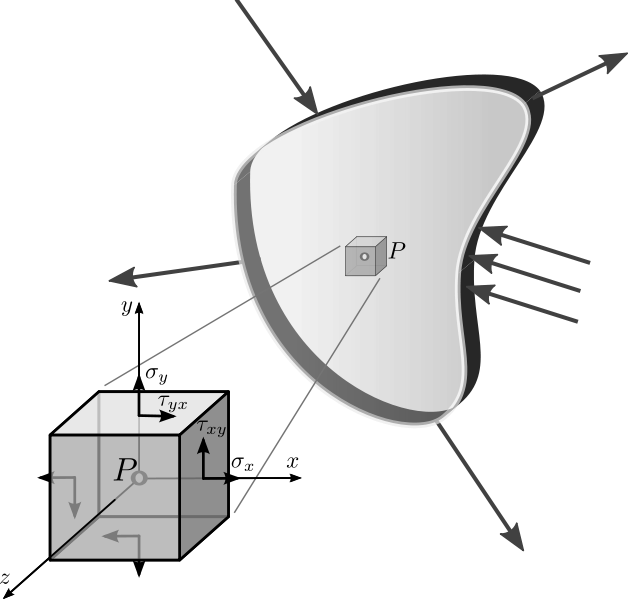
\includegraphics[scale=0.35]{src/ch2/plane_stress.png}
\captionof{figure}{Esfuerzo plano}
\label{fig:fg1}
\end{center}

Entonces, las relaciones esfuerzo deformación se reducen a:

\begin{equation}
\vec{\varepsilon} = [C] \vec{\sigma} + \vec{\varepsilon_0}
\end{equation}

donde:

\begin{equation}
\vec{\varepsilon} = 
\left\{\begin{matrix}
\varepsilon_{xx} \\ \varepsilon_{yy} \\ \varepsilon_{xy}
\end{matrix}\right\}
\end{equation}

\begin{equation}
\vec{\sigma} = 
\left\{\begin{matrix}
\sigma_{xx} \\ \sigma_{yy} \\ \sigma_{xy}
\end{matrix}\right\}
\end{equation}

\begin{equation}
[C] = \frac{1}{E}
\left[\begin{matrix}
1 & -\nu & 0 \\
-\nu & 1 & 0 \\
0 & 0 & 2(1+\nu) \\
\end{matrix}\right]
\end{equation}

\begin{equation}
\vec{\varepsilon_0} = 
\left\{\begin{matrix}
\varepsilon_{xx_0} \\ \varepsilon_{yy_0} \\ \varepsilon_{xy_0}
\end{matrix}\right\} =
\alpha T 
\left\{\begin{matrix}
1 \\ 1 \\ 0 \\
\end{matrix}\right\}
\end{equation}

En el caso de deformaciones térmicas,

\begin{equation}
\vec{\sigma} = [D] (\vec{\varepsilon} - \vec{\varepsilon_0}) = 
[D] \vec{\varepsilon} - 
\frac{E\alpha T}{1-\nu} 
\left\{\begin{matrix}
1 \\ 1 \\ 0 \\
\end{matrix}\right\}
\end{equation}

Con, 

\begin{equation}
[D] = \frac{E}{1-\nu^2}
\left[\begin{matrix}
1 & \nu & 0 \\
\nu & 1 & 0 \\
0 & 0 & \frac{1-\nu}{2} \\
\end{matrix}\right]
\end{equation}

En el caso de esfuerzo plano la componente de la deformación en el plano $z$, será diferente de cero, debido al 
efecto del coeficiente de Poisson, estando dada  por la expresión:

\begin{equation}
\varepsilon_{zz} = -\frac{\nu}{E} (\sigma_{xx} + \sigma_{yy}) + \alpha T = 
\frac{-\nu}{1-\nu} (\varepsilon_{xx} + \varepsilon_{yy}) +  
\frac{1+\nu}{1-\nu} \alpha T
\end{equation}

Mientras que, 

\begin{equation}
\varepsilon_{yz} = \varepsilon_{zx} = 0
\end{equation}


\subsubsection{Deformación plana}

La consideración de deformación plana es aplicable para sólidos largos y cuya geometría y cargas no varían de 
manera significativa en la dirección longitudinal.\\

En este caso las ecuaciones de esfuerzo-deformación tridimensional se reducen a:

\begin{equation}
\vec{\varepsilon} = [C] \vec{\sigma} + \vec{\varepsilon_0}
\end{equation}

donde:

\begin{equation}
\vec{\varepsilon} = 
\left\{\begin{matrix}
\varepsilon_{xx} \\ \varepsilon_{yy} \\ \varepsilon_{xy}
\end{matrix}\right\}
\end{equation}

\begin{equation}
\vec{\sigma} = 
\left\{\begin{matrix}
\sigma_{xx} \\ \sigma_{yy} \\ \sigma_{xy}
\end{matrix}\right\}
\end{equation}

\begin{equation}
[C] = \frac{1+\nu}{E}
\left[\begin{matrix}
1-\nu & -\nu & 0 \\
-\nu & 1-\nu & 0 \\
0 & 0 & 2 \\
\end{matrix}\right]
\end{equation}

\begin{equation}
\vec{\varepsilon_0} = 
\left\{\begin{matrix}
\varepsilon_{xx_0} \\ \varepsilon_{yy_0} \\ \varepsilon_{xy_0}
\end{matrix}\right\} =
(1+\nu) \alpha T 
\left\{\begin{matrix}
1 \\ 1 \\ 0 \\
\end{matrix}\right\}
\end{equation}

En el caso de deformaciones térmicas,

\begin{equation}
\vec{\sigma} = [D] (\vec{\varepsilon} - \vec{\varepsilon_0}) = 
[D] \vec{\varepsilon} - 
\frac{E\alpha T}{1-2\nu} 
\left\{\begin{matrix}
1 \\ 1 \\ 0 \\
\end{matrix}\right\}
\end{equation}

Con, 

\begin{equation}
[D] = \frac{E}{(1+\nu)(1-2\nu)}
\left[\begin{matrix}
1-\nu & \nu & 0 \\
\nu & 1-\nu & 0 \\
0 & 0 & \frac{1-2\nu}{2} \\
\end{matrix}\right]
\end{equation}

\begin{center}
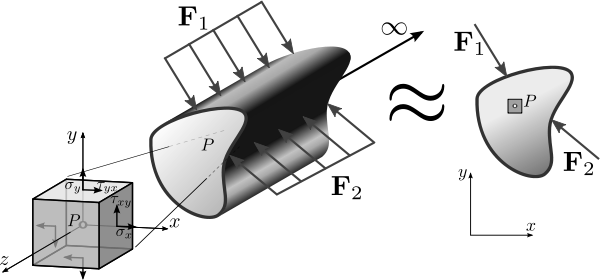
\includegraphics[scale=0.55]{src/ch2/plane_strain.png}
\captionof{figure}{Deformación plana}
\label{fig:fg2}
\end{center}

El componente de esfuerzo en la dirección $z$ no será nulo debido a los efectos del coeficiente de Poisson, y está 
dado por:

\begin{equation}
\sigma_{zz} = \nu(\sigma_{xx}+\sigma_{yy}) - E \alpha T
\end{equation}

y, 

\begin{equation}
\sigma_{yz} = \sigma_{zx} = 0
\end{equation}

\subsection{Relaciones deformación-desplazamiento}

La forma deformada de un cuerpo elástico bajo una determinada configuración de cargas y distribución de temperaturas 
pueden ser descritas completamente por tres componentes de desplazamiento $u, v$ y $w$ paralelas a las direcciones 
$x, y$ y $z$ respectivamente. En general, cada una de estas componentes $u,v$ y $w$ es una función de las 
coordenadas $x,y$ y $z$. Las deformaciones inducidas en el sólido pueden ser expresadas en términos de los 
desplazamientos $u,v$ y $w$.\\

Si los desplazamientos se consideran muy pequeños, la deformaciones pueden ser expresadas como:

\begin{subequations}
\begin{eqnarray}
\varepsilon_{xx} = \frac{du}{dx} \\
\varepsilon_{yy} = \frac{dv}{dy} \\
\varepsilon_{zz} = \frac{dw}{dz} \\
\varepsilon_{xy} = \frac{du}{dy} + \frac{dv}{dx} \\
\varepsilon_{yz} = \frac{dw}{dy} + \frac{dv}{dz} \\
\varepsilon_{zx} = \frac{du}{dz} + \frac{dw}{dx} \\
\end{eqnarray}
\end{subequations}

\subsection{Plasticidad}

La teoría de plasticidad estudia la fluencia de materiales bajo estados de esfuerzos complejos. Permite 
conocer si un material cederá bajo ciertas condiciones de esfuerzo y determinar el cambio en la forma o 
geometría en caso de que la fluencia ocurra. También permite usar datos de ensayos de tensión para predecir 
el endurecimiento por carga durante la deformación bajo complejos estados de esfuerzo. Estas relaciones 
son parte fundamental de los códigos de computadora utilizados para predecir la capacidad de una estructura 
para absorber impactos, así como en procesos de formado o estampado que involucran la deformación plástica de 
placas metálicas.

\subsubsection{Criterio de fluencia}

Un criterio de fluencia es una expresión matemática propuesta del estado de esfuerzo que causará la fluencia. La forma más general es:

\begin{equation}
f(\sigma_x,\sigma_y, \sigma_z, \tau_{yz}, \tau_{zx}, \tau_{xy} ) = C 
\end{equation}

Para materiales isotrópicos esto puede ser expresado en términos de los esfuerzos principales como:

\begin{equation}
f(\sigma_1,\sigma_2,\sigma_3 )=C
\end{equation}

Para la mayoría de los metales dúctiles isotrópicos comúnmente se hacen las siguientes consideraciones:

\begin{itemize}
\item El esfuerzo de fluencia en tensión y compresión es el mismo.
\item El volumen permanece constante durante la deformación plástica
\item La magnitud del esfuerzo normal promedio, no afecta la fluencia.
\end{itemize}

\begin{equation}
\sigma_m=\frac{\sigma_1+\sigma_2+\sigma_3}{3}
\end{equation}

La consideración que la fluencia es independiente de $\sigma_m$ es razonable porque la deformación usualmente ocurre por deslizamiento o mecanismos de corte. Por lo tanto los criterios de fluencia para materiales isotrópicos tienen la forma:

\begin{equation}
f[(\sigma_2-\sigma_3 ),(\sigma_3-\sigma_1 ),(\sigma_1-\sigma_2 )] = C
\end{equation}

\subsubsection{Criterio de Tresca}

El criterio más simple es uno de los primero propuestos por Tresca. Afirma que la cedencia ocurrirá cuando el máximo 
esfuerzo cortante alcance un valor crítico. El máximo esfuerzo cortante viene dado por:

\begin{equation}
\tau_{max} = \frac{\sigma_{max}-\sigma_{min}}{2}
\end{equation}

entonces, el criterio de Tresca puede expresarse como:

\begin{equation}
\sigma_{max} - \sigma_{min} = C
\end{equation}

Si se mantiene la convención de que $ \sigma_1 \me \sigma_2 \me \sigma_3 $, puede reescribirse lo anterior como:

\begin{equation}\label{eq:ec1}
\sigma_1 - \sigma_3 = C
\end{equation}

La constante C puede ser encontrada mediante un ensayo de tensión uniaxial. En un ensayo de tensión, 
$\sigma_2 = \sigma_3 = 0$ y la cedencia $\sigma_1 = Y$, donde $Y$ es el esfuerzo de fluencia. Sustituyendo 
en $C=Y$ en la ecuación \ref{eq:ec1}. Por lo tanto el criterio de Tresca puede ser expresado como:

\begin{equation}\label{eq:ec2}
\sigma_1 - \sigma_3 = Y
\end{equation}

Para cortante puro, $ \sigma_1 = -\sigma_3 = k$, donde $k$ es esfuerzo de fluencia por cortante. Sustituyendo 
$ k = Y/2 $ en la ecuación \ref{eq:ec2}, entonces:

\begin{equation}
\sigma_1 - \sigma_3 = 2k = C
\end{equation}

\subsubsection{Criterio de Von Mises}

El efecto del esfuerzo principal medio puede ser incluido asumiendo que la fluencia depende de la raíz cuadrada 
del promedio de los diámetros de los tres círculos de Mohr. Este es el criterio de Von Mises, el cual puede ser 
expresado como:

\begin{equation} \label{eq:ec3}
\left\{ [(\sigma_2-\sigma_3)^2 + (\sigma_3-\sigma_1 )^2 + (\sigma_1-\sigma_2 )^2]/3 \right\}^{1/2} = C
\end{equation}

Como cada término está elevado al cuadrado, la convención $\sigma_1 \me \sigma_2 \me \sigma_3$ no es necesaria. 
La constante del material, $C$, puede ser evaluada mediante un ensayo de tensión uniaxial. En la fluencia, 
$\sigma_1 = Y$ y $\sigma_2 = \sigma_3 = 0$. Sustituyendo, $[0^2 + (-Y)^2 + Y^2]/3 = C^2$, o 
$C = (2/3)^{1/3} Y $, entonces, la ecuación usualmente se escribe como:

\begin{equation}\label{eq:ec4}
(\sigma_2-\sigma_3)^2 + (\sigma_3-\sigma_1 )^2 + (\sigma_1-\sigma_2 )^2 = 2Y^2
\end{equation}

Para cortante puro, $\sigma_1 = -\sigma_3 = k$ y $\sigma_2=0$. Sustituyendo en la ecuación \ref{eq:ec4}, 
$ (-k)^2 + [ (-k)-k ]^2 + k^2 = 2Y^2 $, entonces:

\begin{equation}\label{eq:ec5}
k = Y/\sqrt{3}
\end{equation}

La ecuación \ref{eq:ec5} puede ser simplificada si uno de los esfuerzos principales es cero (condición de esfuerzo plano). 
Sustituyendo $\sigma_3 = 0$, $\sigma_1^2 + \sigma_2^2 - \sigma_1 \sigma_2 = Y^2$, el cual es una elipse. Con la 
consiguiente sustitución de $\alpha = \sigma_2/\sigma_1$,

\begin{equation}
\sigma_1 = Y/(1-\alpha+\alpha^2)^{1/2}
\end{equation}


\subsection{Ecuaciones de equilibrio}

\subsubsection{Equilibrio externo}

Si un sólido está en equilibrio bajo ciertas condiciones de carga, las fuerzas reactivas y momentos desarrollados en 
los puntos de soporte deben balancear las fuerzas y momentos externos aplicados. Haciendo referencia a la figura 
\ref{fig:externalforces}, sean $\phi_x, \phi_y, \phi_z$ las fuerzas de cuerpo, $\Phi_x, \Phi_y, \Phi_z$ las 
fuerzas de superficie, $P_x, P_y, P_z$ las fuerzas concentradas externas, y $Q_x, Q_y, Q_z$ los momentos externos 
aplicados. Entonces, las ecuaciones de equilibrio externo pueden establecerse como:

\begin{eqnarray}
\int_S \Phi_x ds + \int_V \phi_x dV + \sum P_x = 0 \nonumber \\
\int_S \Phi_y ds + \int_V \phi_y dV + \sum P_y = 0 \\
\int_S \Phi_z ds + \int_V \phi_z dV + \sum P_z = 0 \nonumber
\end{eqnarray}

\begin{center}
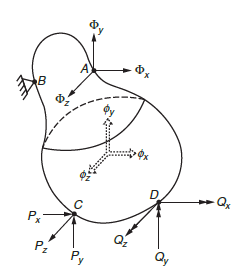
\includegraphics[scale]{src/ch2/equillibrium_force.png}
\captionof{figure}{Fuerzas de equilibrio externo}
\label{fig:externalforces}
\end{center}

Para el equilibrio de momentos:

\begin{eqnarray}
\int_S (\Phi_zy - \Phi_{y}z) ds + \int_V (\phi_zy - \phi_{y}z) dV + \sum Q_x = 0 \nonumber \\
\int_S (\Phi_x z - \Phi_z x) ds + \int_V (\phi_x z - \phi_z x) dV + \sum Q_y = 0 \\
\int_S (\Phi_{y}x - \Phi_x y) ds + \int_V (\phi_{y}x - \phi_x y) dV + \sum Q_z = 0 \nonumber
\end{eqnarray}

Donde $S$ es la superficie y $V$ el volumen del cuerpo sólido.


\subsubsection{Equilibrio interno}

Debido a las aplicación de cargas, se desarrollan esfuerzos dentro del sólido. Si consideramos 
un elemento de material dentro del sólido, este debería estar en equilibrio debido a esos 
esfuerzos internos desarrollados.\\

Teoricamente, el estado de esfuerzos en cualquier punto de un cuerpo cargado está completamente definido 
en términos de nueve componentes de esfuerzo: $\sigma_{xx}, \sigma_{yy}, \sigma_{zz}, \sigma_{xy}, \sigma_{yx}, 
\sigma_{yz}, \sigma_{zy}, \sigma_{zx}, \sigma_{xz} $, donde los primeros tres son las componentes normales y los restantes 
son esfuerzos cortantes. Las ecuaciones de equilibrio interno relativas a los nueve componentes de esfuerzo pueden ser 
obtenidas considerando el equilibrio de momentos y fuerzas actuando en el volumen elemental mostrado en 
la figura \ref{fig:internalforces}. El equilibrio de momentos alrededor de los ejes $x,y,z$, asumiendo que no existen 
momentos en el sólido, derivan en las siguientes relaciones:

\begin{equation}
\sigma_{yx} = \sigma_{xy}, \,\,\,\, \sigma_{zy} = \sigma_{yz}, \,\,\,\, \sigma_{xz} = \sigma_{zx}
\end{equation}

\begin{center}
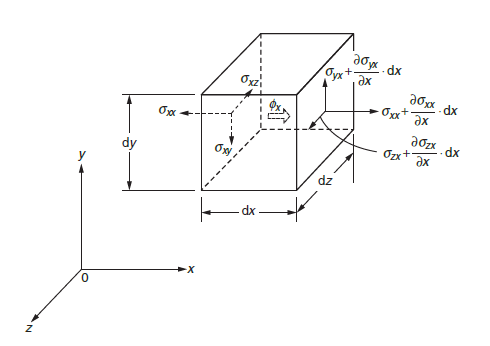
\includegraphics[scale]{src/ch2/internal_force.png}
\captionof{figure}{Fuerzas de equilibrio interno}
\label{fig:internalforces}
\end{center}

Estas ecuaciones muestran que el estado de esfuerzos en cualquier punto puede ser completamente definido por 
los seis componentes $\sigma_{xx}, \sigma_{yy}, \sigma_{zz}, \sigma_{xy}, \sigma_{yz}, \sigma_{zx} $. 
El equilibrio de fuerzas en las direcciones $x,y,z$ proporcionan las siguientes ecuaciones diferenciales de 
equilibrio:

\begin{eqnarray}
\frac{\partial \sigma_{xx}}{\partial x} + \frac{\partial \sigma_{xy}}{\partial y} + 
\frac{\partial \sigma_{zx}}{\partial z} + \phi_{x} = 0 \nonumber \\
\frac{\partial \sigma_{xy}}{\partial x} + \frac{\partial \sigma_{yy}}{\partial y} + 
\frac{\partial \sigma_{yz}}{\partial z} + \phi_{y} = 0 \\
\frac{\partial \sigma_{zx}}{\partial x} + \frac{\partial \sigma_{yz}}{\partial y} + 
\frac{\partial \sigma_{zz}}{\partial z} + \phi_{z} = 0 \nonumber
\end{eqnarray}

donde $\phi_x, \phi_y$ y $\phi_z$, son las fuerzas de cuerpo por unidad de volumen actuando a lo largo 
de las direcciones $x,y$ y $z$, respectivamente.\\

Para un problema bidimensional, existen solamente tres componentes de esfuerzo independientes, 
$(\sigma_{xx},\sigma_{yy},\sigma_{xy})$ y las ecuaciones de equilibrio se reducen a:

\begin{eqnarray}
\frac{\partial \sigma_{xx}}{\partial x} + \frac{\partial \sigma_{xy}}{\partial y} + \phi_x = 0 \nonumber \\
\frac{\partial \sigma_{xy}}{\partial x} + \frac{\partial \sigma_{yy}}{\partial y} + \phi_y = 0 
\end{eqnarray}

En problemas unidimensionales, sólo estará presente un componente de esfuerzo: $\sigma_{xx}$. Entonces, 
las ecuaciones de equilibrio se reducen a:

\begin{equation}
\frac{\partial \sigma_{xx}}{\partial x} + \phi_x = 0
\end{equation}


\section{El método de los elementos finitos}

\subsection{Generalidades del método}

En el método de elementos finitos se considera un cuerpo continuo o sólido, como un ensamble de pequeñas subdivisiones llamadas elementos finitos. Estos elementos están interconectados a través de nodos comunes. Debido a que la variación real de las variables de campo (desplazamientos, esfuerzos, temperaturas, etc.) se desconoce en el continuo, se asume que la variación de estas en el modelo de elemento finito puede ser aproximada por una simple función. Estas funciones de aproximación, también llamadas modelos de interpolación, son definidas en términos de los valores nodales de las variables de campo.\\

En general, el método de los elementos finitos, consiste en formular un sistema de ecuaciones (ecuaciones de equilibrio) para el sistema continuo que ha sido discretizado, donde las incógnitas suelen ser los valores nodales de las variables de campo. Luego, se resuelve este sistema de ecuaciones, con las consideraciones correspondientes a las condiciones de frontera o valores iniciales que simplifiquen el modelo original. La siguiente ecuación muestra, en notación matricial, el sistema de ecuaciones resuelto en una formulación de elemento finito.

\begin{equation}
\bm{\left[K\right] \vec{u} = \vec{P}}
\end{equation}

Donde $\bm{[K]}$ es la matriz global de rigidez, $\bm{\vec{u}}$ es el vector de desplazamientos nodales y $\bm{\vec{P}}$ el vector de fuerzas nodales en el sistema.\\

Para problemas lineales, el vector $\bm{\vec{u}}$ puede ser resuelto de manera sencilla, mediante procedimientos básicos del álgebra lineal. Sin embargo, para problemas no lineales, la solución tiene que ser obtenida mediante una secuencia de pasos, en el cual cada uno de estos implica la modificación de la matriz de rigidez $\bm{[K]}$ y/o el vector global de carga $\bm{\vec{P}}$.

\subsection{Análisis dinámico}

En problemas de análisis dinámico, desplazamientos, velocidades, deformaciones, esfuerzos y cargas 
son dependientes del tiempo. El procedimiento de solución por elemento finito implica las siguientes 
consideraciones o pasos.\\

Primeramente, como en el caso estático, se debe idealizar el sólido en módelo de elementos finitos. 
Luego, se asume que los desplazamientos del elemento $e$ se pueden definir como:

\begin{equation}\label{eq:dynec1}
\vec{U}(x,y,z,t) = 
\left\{ \begin{matrix}
u(x,y,z,t) \\ v(x,y,z,t) \\ w(x,y,z,t) \\
\end{matrix} \right\} = 
[N(x,y,z)] \vec{Q}^{(e)}(t)
\end{equation}

Donde $\vec{U}$ es el vector de desplazamientos, $[N]$ es la matriz de funciones de forma, y $\vec{Q}_{(e)}$ 
es el vector de desplazamientos nodales que se considera como una función del tiempo.\\

Derivando las matrices de rigidez y masa características, además del vector de cargas, de la ecuación \ref{eq:dynec1} 
se pueden expresar las deformaciones como:

\begin{equation}
\vec{\varepsilon} = [B] \vec{Q}_^{(e)}
\end{equation}

y los esfuerzos como,

\begin{equation}
\vec{\sigma} = [D] \vec{\varepsilon} = [D][B] \vec{Q}^{(e)}
\end{equation}

Derivando la ecuación \ref{eq:dynec1} con respecto al tiempo, el campo de velocidades puede ser obtenido: 

\begin{equation}
\dot{\vec{U}}(x,y,z,t) = [N(x,y,z)]\dot{\vec{Q}}^{(e)} (t)
\end{equation}

donde $\dot{\vec{Q}}^{(e)}$ es el vector de velocidades nodales. Para derivar las ecuaciones de movimiento de 
una estructura, podemos usar las ecuaciones de Lagrange (\ref{eq:dynec1}) o el principio de Hamilton. Las 
ecuaciones de Lagrange están dadas por:

\begin{equation}
\frac{d}{dt} \left\{ \frac{\partial L}{\partial \dot{Q}} \right\}- 
\left\{ \frac{\partial L}{\partial Q} \right\} + 
\left\{ \frac{\partial R}{\partial \dot{Q}} \right\} = \{0\}
\end{equation}

donde,

\begin{equation}
L = T - \pi_p
\end{equation}

es llamada función Lagrangiana, T es la energía cinética, $\pi_p$ es la energía potencial, $R$ es 
la función de disipación, $Q$ es el desplazamiento nodal, y $\dot{Q}$ es la velocidad nodal.
La energía cinética y la energía potencial de un elemento $(e)$ puede ser expresada como:

\begin{equation}
T^{(e)}	= \frac{1}{2} \iiint_{V^{(e)}} \rho \dot{\vec{U}}^T \dot{\vec{U}} dV
\end{equation}

y,

\begin{equation}
\pi_p^{(e)} = \frac{1}{2} 
\iiint_{V^e} \vec{\varepsilon}^T \vec{\sigma} dV  - 
\iint_{S_1^e} \vec{U}^T \vec{\Phi} dS_1  - 
\iiint_{V^e} \vec{U}^T \vec{\Phi} dV
\end{equation}

donde $V^{(e)}$ es el volumen, $\rho$ es la densidad, $\dot{\vec{U}}$ es el vector de las velocidades del elemento $(e)$. 
Asumiendo la existencia de fuerzas disipativas proporcionales a las velocidades relativas, la función de disipación del 
elemento $(e)$ puede ser expresado como:

\begin{equation}
R^{(e)} = \frac{1}{2} \iiint_{V^{(e)}} \mu \dot{\vec{U}}^T \dot{\vec{U}} dV
\end{equation}

Donde $\mu$ es el coeficiente de amortiguamiento. Las expresiones para $T$, $\pi_p$ y $R$ pueden 
ser reescritas como:

\begin{equation}
T = \sum\limits_{e=1}^{E} T^{(e)} = \frac{1}{2} \dot{\vec{Q}}^T
\left[
\sum\limits_{e=1}^{E} \iiint\limits_{V^{(e)}} \rho [N]^T [N] dV
\right]
\dot{\vec{Q}}
\end{equation}

\begin{equation}
\pi_p = \sum\limits_{e=1}^{E} \pi_p^{(e)} = \frac{1}{2} \dot{\vec{Q}}^T
\left[
\sum\limits_{e=1}^{E} \iiint\limits_{V^{(e)}} [B]^T [D] [B] dV
\right] \vec{Q} - 
\vec{Q}^T 
\left(
\sum\limits_{e=1}^{E} \iint\limits_{S_1^{(e)}} [N]^T \vec{\Phi}(t) dS_1   + 
\iiint\limits_{V^{(e)}} [N]^T \vec{\Phi}(t) dV 
\right) -
\vec{Q}^T \vec{P}_c (t)
\end{equation}


\begin{equation}
R = \sum\limits_{e=1}^{E} R^{(e)} = \frac{1}{2} \dot{\vec{Q}}^T
\left[
\sum\limits_{e=1}^{E} \iiint\limits_{V^{(e)}} \mu [N]^T [N] dV 
\right]
\dot{\vec{Q}}
\end{equation}

Donde $\vec{Q}$ es el vector global de desplazamientos, $\dot{\vec{Q}}$ es el vector global de velocidades, 
y $\vec{P}_c$ es el vector de fuerzas concentradas nodales en la estructura del sólido. Las matrices que 
implican las integrales se pueden definir como:

\begin{equation}
[M^{(e)}] = \iiint\limits_{V^{(e)}} \rho [N]^T [N] dV
\end{equation}

\begin{equation}
[K^{(e)}] = \iiint\limits_{V^{(e)}} [B]^T [D] [B] dV
\end{equation}

\begin{equation}
[C^{(e)}] = \iiint\limits_{V^{(e)}} \mu [N]^T [N] dV
\end{equation}

\begin{equation}
[P_s^{(e)}] = \iint\limits_{S_1^{(e)}} [N]^T \vec{\Phi} dS_1
\end{equation}

\begin{equation}
[P_b^{(e)}] = \iint\limits_{V^{(e)}} [N]^T \vec{\Phi} dV
\end{equation}

Una vez se tienen las matrices características individuales, se deben  ensamblar las matrices globales y 
obtener las ecuaciones totales de movimiento.

\begin{equation}
T = \frac{1}{2} \dot{\vec{Q}}^T [M] \dot{\vec{Q}}
\end{equation}

\begin{equation}
\pi_p = \frac{1}{2} \dot{\vec{Q}}^T [K] \vec{Q} - \vec{Q}^T \vec{P}
\end{equation}

\begin{equation}
R = \frac{1}{2} \dot{\vec{Q}}^T [C] \dot{\vec{Q}}
\end{equation}

donde, 

$$
[M] = \sum\limits_{e=1}^{E} [M^{(e)}]
$$
$$[K] = \sum\limits_{e=1}^{E} [K^{(e)}]$$
$$[C] = \sum\limits_{e=1}^{E} [C^{(e)}]$$
$$
\vec{P}(t) = \sum\limits_{e=1}^{E} 
\left(
P_s^{(e)}(t) + P_b^{(e)}(t) 
\right)
+ P_c (t)
$$

Obtenemos la ecuación de movimiento del sólido:

\begin{equation}
[M] \ddot{\vec{Q}}(t) + [C] \dot{\vec{Q}}(t) + [K] \vec{Q} (t) = \vec{P} (t)
\end{equation}

Donde \ddot{\vec{Q}} es el vector de las aceleraciones nodales en el sistema global. Si se ignora 
las ecuación de movimiento puede ser escrita como:

\begin{equation}
[M] \ddot{\vec{Q}} + [K] \vec{Q} = \vec{P}
\end{equation}



\subsection{Solución implícita vs explícita}

De manera más general, el sistema de ecuaciones que describe un modelo de elemento finito en un determinado tiempo, se puede escribir como:

\begin{equation}
M\ddot{u} + C\dot{u} ̇+ f_{int} = f_{ext}
\end{equation}

Donde $C\dot{u}$ representa las fuerzas viscosas, mismas que deben incluirse cuando el sistema esté amortiguado artificialmente.\\ 
Existen, de manera general, dos tipos de métodos para resolver ecuaciones diferenciales  en problemas dependientes del tiempo: integración implícita e integración explícita. El método implícito de integración en el tiempo puede ser expresado como:

\begin{equation}
u_{n+1}=f(\dot{u}_{n+1},\ddot{u}_{n+1},u_n,\dot{u}_n,…)
\end{equation}

y el método explícito como:

\begin{equation}
u_{n+1}=f(u_n,\dot{u}_n,\ddot{u}_n,u_{n-1},\dot{u}_{n-1},…)
\end{equation}

El método implícito requiere conocer las derivadas temporales en el paso n+1, las cuales son desconocidas, mientras el método explícito está basado en los valores conocidos en el paso n. Si el problema es no lineal, el método implícito necesita un procedimiento iterativo para determinar los nuevos desplazamientos. Con el método explícito los nuevos desplazamientos se determinan directamente de los valores conocidos en pasos previos, evitando el uso de iteraciones adicionales.\\

La simulación de estampados se caracteriza por las diversas no linealidades presentes, debidas al material, y a los contactos entre los diversos cuerpos analizados. Sin embargo, usando la integración explícita estas no linealidades pueden ser tratadas sin mayores problemas. Por ello, en la mayoría de las simulaciones de estampados suelen ser conveniente el uso de algoritmos de integración explícita.

\section{Teoría de contactos}

\subsection{Introducción}

Considere el movimiento dependiente del tiempo de dos cuerpos ocupando las regiones $B^1$ y $B^2$ 
en su configuración deformada en el tiempo cero. Asuma que la intersección

$$
B^1 \cap B^2 = \emptyset
$$

es satisfecha. Sean $\partial B^1$ y $\partial B^1$ quienes denotan las fronteras de $B^1$ y $B^2$ 
respectivamente. En un tiempo posterior, estos cuerpos ocupan las regiones $b^1$ y $b^2$ delimitadas 
por $\partial b^1$ y $\partial b^2$ como se muestra en la figura \ref{fig:refanddef}. Debido a que la 
configuración deformada no puede penetrar:

$$
\left( b^1 - \partial b^1 \right) \cap b^2 = \emptyset
$$

Mientras $\left( \partial b^1 \cap \partial b^2 \right) = \emptyset$, las ecuaciones de movimiento 
permanecen desacopladas. En las anteriores y siguientes ecuaciones, el superíndice derecho $\alpha$ 
$(=1,2)$ denota el cuerpo al cual la cantidad hace referencia.

\begin{center}
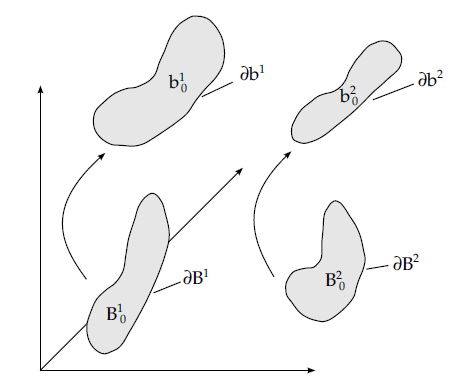
\includegraphics[scale=0.6]{src/ch2/ref_and_def.png}
\captionof{figure}{Configuración de referencia y deformada}
\label{fig:refanddef}
\end{center}

Antes de dar una descripción detallada de la teoría de contactos, algunos cuestiones adicionales 
referentes a la terminología deben ser agregadas. Las superficies $\partial b^1$ y $\partial b^2$ 
de los cuerpos discretizados $b^1$ y $b^2$ vienen a ser las superficies \textit{maestra} 
y \textit{esclava}, respectivamente. La selección de las superficies maestra y esclava es 
arbitraria cuando el tratamiento simétrico de penalización es utilizado. De lo contrario, 
la superficie de malla más \textit{burda} debe ser elegida como maestra a menos que 
exista una gran diferencia en las densidades de masa, en cuyo caso se recomienda definir 
como superficie maestra al del material con mayor densidad de masa. Los puntos nodales 
que definen $\partial b^1$ son llamados nodos maestros y los nodos que definen $\partial b^2$ 
son llamados nodos esclavos. Cuando $\left( \partial b^1 \cap \partial b^2 \right) \neq \emptyset$, 
las restricciones son impuestas para prevenir la penetración. Los superíndices derechos se 
utilizan cuando una variable se refiere tanto a la superficie maestra $\partial b^1$ o 
a la sueperficie esclava $\partial b^2$, consecuentemente estos superíndices se descartan 
en el desarrollo siguiente.

\subsection{\textit{Slave search}}

Esta búsqueda encuentra para cada nodo esclavo su punto más cercano en la superficie maestra. 
Las líneas dibujadas de un nodo esclavo a sus puntos más cercanos serán perpendiculares a la 
superficie maestra, a menos que el punto se encuentre en la intersección de dos segmentos 
maestros, donde un segmento está definido a ser un elemento de superficie de 3 o 4 nodos.\\

Considere un nodo esclavo, $n_s$, deslizándose en una superficie maestra suave a tramos y 
asuma que una búsqueda de la superficie maestra ha encontrado el nodo maestro, $m_s$, 
situado cerca de $n_s$. La figura \ref{fig:slave_search} representa una porción 
de una superficie maestra con nodos referenciados como $m_s$ y $n_s$. Si $m_s$ 
y $n_s$ no coinciden, para $n_s$ por lo general se puede demostrar que se encuentra 
en un segmento $s_1$  mediante el siguiente test:

\begin{equation}
(\mathbf{c_i} x \mathbf{s}) \cdot (\mathbf{c_i} x \mathbf{c_{i+1}}) > 0
\end{equation}

\begin{equation}
(\mathbf{c_i} x \mathbf{s}) \cdot (\mathbf{s} x \mathbf{c_{i+1}}) > 0
\end{equation}

donde el vector $\mathbf{c_i}$ y $\mathbf{c_{i+1}}$

\begin{center}
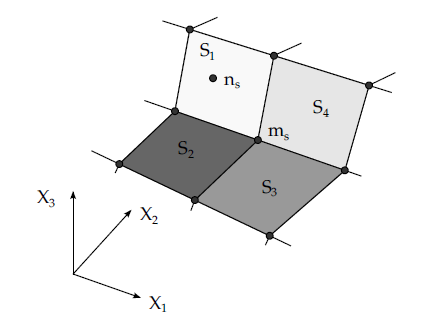
\includegraphics[scale=0.6]{src/ch2/slave_search.png}
\captionof{figure}{Slave search}
\label{fig:slave_search}
\end{center}




\subsection{Algoritmo de contacto superficie-superficie}

Este implica un enfoque simétrico de dos pasos con un parámetro 
de partición, $\beta$, que se establece entre la unidad positiva y negativa, donde $\beta=1$ 
y $\beta=-1$ corresponden a tratamiento de una forma con la superficie \textit{maestra} 
acumulando masa y fuerzas de la superficie \textit{esclava} (para $\beta = 1$) y viceversa 
(para $\beta = -1$). ~\cite{lsdyna-manual} \\ 

En este enfoque de restricción las aceleraciones, velocidades y desplazamientos se actualizan 
primero a una configuración de prueba sin tener en cuenta las interacciones. Después de la 
actualización, una fuerza de penetración es calculada para el nodo esclavo como una función 
de la distancia de penetración $\Delta L$:

$$
\mathbf{\f_p} = \frac{m_s \Delta L}{\Delta t^2}\mathbf{n},
$$

Donde $\mathbf{n}$ es el vector normal a la superficie maestra.\\

Se desea que la respuesta de la componente normal del vector de aceleración del nodo esclavo, 
$\mathbf{a_s}$, de un nodo esclavo residiendo en un segmento maestro $k$ sea consistente con 
el movimiento del segmento maestro en su porción de contacto $(s_c,t_c)$, por ejemplo:

$$
a_s = \phi_1 (s_c,t_c) a_{nk}^1 + \phi_2 (s_c,t_c) a_{nk}^2 + \phi_3 (s_c,t_c) a_{nk}^3 + \phi_4 (s_c,t_c) a_{nk}^4
$$

Para cada nodo esclavo en contacto y penetrando a través de la superficie maestra en 
su configuración de prueba, su masa nodal y fuerza de penetración dadas por la ecuación 
[REVISAR (Poner aquí referencia)] es acumulada a una masa y vector de fuerza global de 
la superficie maestra.

$$
\left(
m_k + \sum_s m_{ks}
\right)
\mathbf{a_{nk}}
=
\sum_s \mathbf{f_{ks}}
$$

donde:

$$
m_{ks} = \phi_k m_s
$$

$$
\mathbf{f_{ks}} = \phi{k} \mathbf{f_s}
$$

Después de resolver la ecuación [REVISAR] para el vector de aceleración, $\mathbf{a_{nk}}$, podemos 
obtener la corrección de aceleración para el nodo esclavo como:

$$
\mathbf{a_{ns}} = \mathbf{a_s} - \frac{f_p}{m_s}
$$

El proceso anterior es repetido después de invertir las definiciones de \textit{maestro-esclavo}. 
En el paso final la corrección final promediada al vector de aceleración es encontrada:

$$
\mathbf{a_n^{final}} = \frac{1}{2} (1-\beta) \mathbf{a_n^{1st pass}} + 
\frac{1}{2} (1-\beta) \mathbf{a_n^{2nd pass}} 
$$

Y se usa para calcular la aceleración final en el tiempo $n+1$

$$
\mathbf{a}^{n+1} = \mathbf{a}^{prueba} + \mathbf{a}_n^{final}
$$

La fricción resiste la velocidad tangencial relativa del nodo esclavo con respecto a 
la superficie maestra. Esta velocidad relativa se expresa como:

$$
\mathbf{v_r} = \mathbf{v_s} - 
\left(
\phi_1 \mathbf{v}_k^1 + \phi_2 \mathbf{v}_k^2 + \phi_3 \mathbf{v}_k^3 + \phi_4 \mathbf{v}_k^4
\right)
$$

la componente normal de la velocidad al segmento maestro:

$$
\mathbf{v_t} = \mathbf{v_r} - (\mathbf{n} \cdot \mathbf{v_r}) \mathbf{n}
$$

Una fuerza tangencial de prueba es calculada que cancelará la velocidad tangencial:

$$
\mathbf{f^{\ast}} = \frac{m_s v_t}{\Delta t}
$$

Donde $v_t$ es la magnitud del vector de velocidad tangencial.

$$
v_t = \sqrt{\mathbf{v}_t \cdot \mathbf{v}_t}
$$

La magnitud de la fuerza tangencial es limitada por la magnitud del producto de la constante de fricción 
de Coulomb con la fuerza normal definido como:

$$
f_n = m_s \mathbf{a}_{ns} \cdot \mathbf{n}
$$

La fuerza limitada es, por lo tanto:

$$
F_y = m |\mathbf{f}_n|
$$

y 

$$
\mathbf{f}^{n+1} = \mathbf{f^{\ast}} \,\,\, if \,\,\, |\mathbf{f^{\ast}}| = F_y
$$

$$
\mathbf{f}^{n+1} = \frac{F_y \mathbf{f^{\ast}}}{|\mathbf{f^{\ast}}|} \,\,\, if \,\,\, |\mathbf{f^{\ast}}| > F_y
$$

Por lo tanto, usando las ecuaciones anteriores la modificiación a la componente de  aceleración tangencial 
del nodo esclavo está dado por:

$$
\mathbf{a_t} = \min\left( \mu \mathbf{a_{nt}} \cdot \mathbf{n} , \frac{|\mathbf{v_s}|}{\Delta t} \right)
$$

el cual debe actuar en la dirección del vector tangencial definido como:

$$
\mathbf{n_t} = \frac{\mathbf{v_t}}{v_t}
$$

Las correcciones a las componentes de aceleración del nodo esclavo y maestro son: 

$$
a_{ts} = a_{t} \mathbf{n_t}
$$

$$
\mathbf{a_{tk}} = - \phi_k \frac{a_s m_s}{m_k} \mathbf{n_t}
$$

El proceso anterior se repite después de invertir la definición de esclavo y maestro. En el 
paso final la corrección final promediada al vector de aceleración está dada por:

$$
\mathbf{a}_t^{final} = \frac{1}{2} \left( 1-\beta \right) \mathbf{a}_t^{1st pass}  + 
\frac{1}{2} \left( 1 + \beta \right) \mathbf{a}_t^{2nd pass} 
$$

y es usado para calcular la aceleración final en el tiempo $n+1$: 

$$
\mathbf{a}^{n+1} = \mathbf{a}^{prueba}  +  \mathbf{a}_n^{final} + \mathbf{a}_t^{final}
$$

Una desventaja significativa del método de restricción respecto al método de penalización 
aparece si un nodo de interfaz está sujeto a una restricción adicional como puntos de 
soldadura, ecuaciones de restricción y cuerpos rígidos. Los cuerpos rígidos pueden 
ser usados con estos algoritmos de contacto si sus movimientos están prescritos como 
en el caso de los procesos de estampado. Para la mayoría de los casos que involucran 
cuerpos rígidos, las ecuaciones anteriores no son directamente aplicables ya que las 
masas nodales locales de los nodos de cuerpos rígidos son usualmente insignificantes. 
Someter los dos lados de una superficie \textit{shell} a este algoritmo de contacto 
también dará lugar a resultados erróneos, ya que un nodo de interfaz no puede 
ser restringido a moverse simultáneamente en dos superficies mutuamente independientes.\\

La mayor ventaja del algoritmo de restricción es que los nodos de interfaz permanecen 
muy cerca de las superficies con las cuales están en contacto. Además, las vibraciones 
elásticas que pueden ocurrir en las formulaciones de penalización son insignificantes 
con la técnica de restricción, evitando además la necesidad de encontrar una constante 
adecuada de penalización.




